\documentclass[tikz,border=10pt]{standalone}

\usepackage{amsmath,amssymb}
\usepackage{tikz}
\usetikzlibrary{arrows.meta,positioning,calc}

\newcommand{\F}{\mathbb{F}}
\newcommand{\C}{\mathbb{C}}
\newcommand{\Z}{\mathbb{Z}}
\newcommand{\Spec}{\operatorname{Spec}}
\newcommand{\ideal}[1]{\langle #1\rangle}
\newcommand{\ol}[1]{\overline{#1}}
\newcommand{\im}{\operatorname{im}}
\newcommand{\Ker}{\operatorname{Ker}}

\begin{document}
	
	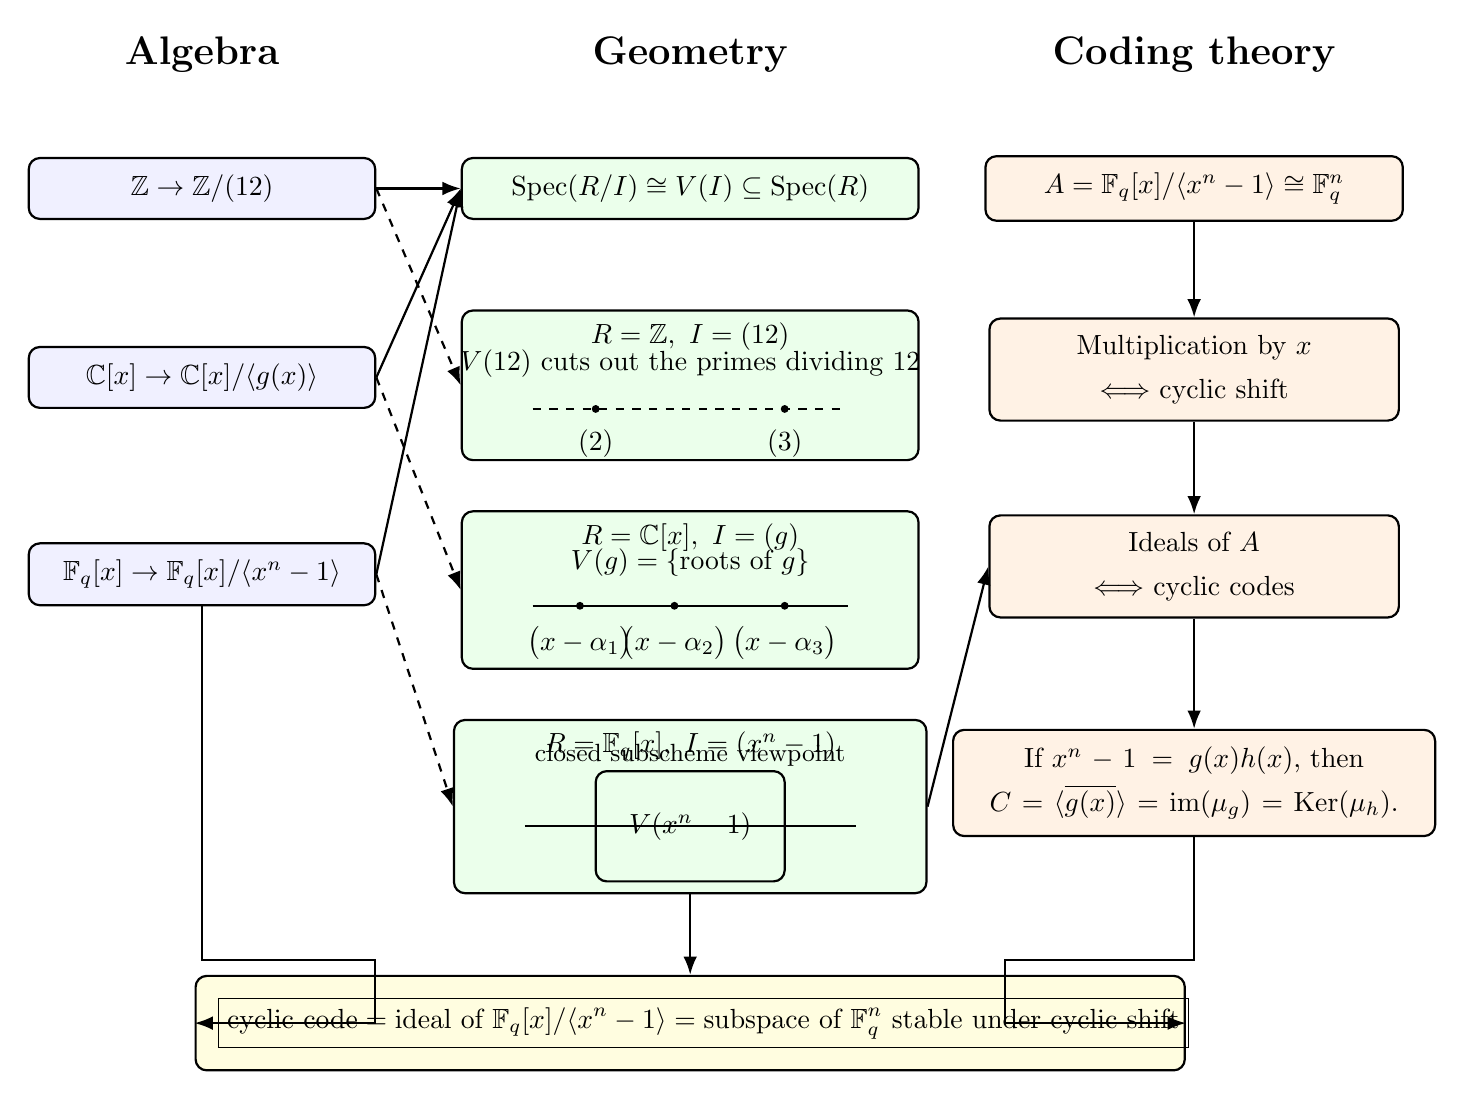
\begin{tikzpicture}[
		>=Latex,
		ringbox/.style={draw, rounded corners, thick, fill=blue!6, align=center, inner sep=6pt},
		geombox/.style={draw, rounded corners, thick, fill=green!8, align=center, inner sep=6pt},
		codebox/.style={draw, rounded corners, thick, fill=orange!10, align=center, inner sep=6pt}
		]
		
		\node[font=\bfseries\Large] at (-6.2,5.3) {Algebra};
		\node[font=\bfseries\Large] at (0,5.3) {Geometry};
		\node[font=\bfseries\Large] at (6.4,5.3) {Coding theory};
		
		% Algebra column
		\node[ringbox, minimum width=4.4cm] (zalg) at (-6.2,3.6) {$\Z \to \Z/(12)$};
		\node[ringbox, minimum width=4.4cm] (calg) at (-6.2,1.2) {$\C[x]\to \C[x]/\ideal{g(x)}$};
		\node[ringbox, minimum width=4.4cm] (falg) at (-6.2,-1.3) {$\F_q[x]\to \F_q[x]/\ideal{x^n-1}$};
		
		% Geometry column
		\node[geombox, minimum width=5.8cm] (specmain) at (0,3.6) {$\Spec(R/I)\cong V(I)\subseteq \Spec(R)$};
		
		\node[geombox, minimum width=5.8cm, minimum height=1.9cm] (zgeo) at (0,1.1) {};
		\node at ($(zgeo.north)+(0,-0.35)$) {$R=\Z,\ I=(12)$};
		\draw[dashed, thick] ($(zgeo.center)+(-2.0,-0.3)$) -- ($(zgeo.center)+(2.0,-0.3)$);
		\filldraw[black] ($(zgeo.center)+(-1.2,-0.3)$) circle (1.2pt);
		\filldraw[black] ($(zgeo.center)+( 1.2,-0.3)$) circle (1.2pt);
		\node[below=4pt] at ($(zgeo.center)+(-1.2,-0.3)$) {$(2)$};
		\node[below=4pt] at ($(zgeo.center)+(1.2,-0.3)$) {$(3)$};
		\node at ($(zgeo.center)+(0,0.28)$) {$V(12)$ cuts out the primes dividing $12$};
		
		\node[geombox, minimum width=5.8cm, minimum height=2.0cm] (cgeo) at (0,-1.5) {};
		\node at ($(cgeo.north)+(0,-0.35)$) {$R=\C[x],\ I=(g)$};
		\draw[thick] ($(cgeo.center)+(-2.0,-0.2)$) -- ($(cgeo.center)+(2.0,-0.2)$);
		\foreach \x/\lab in {-1.4/\alpha_1,-0.2/\alpha_2,1.2/\alpha_3}{
			\filldraw[black] ($(cgeo.center)+(\x,-0.2)$) circle (1.2pt);
			\node[below=4pt] at ($(cgeo.center)+(\x,-0.2)$) {$\bigl(x-\lab\bigr)$};
		}
		\node at ($(cgeo.center)+(0,0.35)$) {$V(g)=\{\text{roots of }g\}$};
		
		\node[geombox, minimum width=6.0cm, minimum height=2.2cm] (fgeo) at (0,-4.25) {};
		\node at ($(fgeo.north)+(0,-0.35)$) {$R=\F_q[x],\ I=(x^n-1)$};
		\draw[thick] ($(fgeo.center)+(-2.1,-0.25)$) -- ($(fgeo.center)+(2.1,-0.25)$);
		\draw[thick, rounded corners] ($(fgeo.center)+(-1.2,0.45)$) rectangle ($(fgeo.center)+(1.2,-0.95)$);
		\node at ($(fgeo.center)+(0,-0.25)$) {$V(x^n-1)$};
		\node at ($(fgeo.center)+(0,0.65)$) {\small closed subscheme viewpoint};
		
		% Coding column
		\node[codebox, minimum width=5.3cm] (Abox) at (6.4,3.6) {$A=\F_q[x]/\ideal{x^n-1}\cong \F_q^n$};
		
		\node[codebox, minimum width=5.2cm] (shiftbox) at (6.4,1.3) {%
			Multiplication by $x$\\[4pt]
			$\Longleftrightarrow$ cyclic shift};
		
		\node[codebox, minimum width=5.2cm] (idealbox) at (6.4,-1.2) {%
			Ideals of $A$\\[4pt]
			$\Longleftrightarrow$ cyclic codes};
		
		\node[codebox, minimum width=6.0cm, text width=5.7cm] (factorbox) at (6.4,-3.95) {%
			If $x^n-1=g(x)h(x)$, then\\[4pt]
			$C=\ideal{\ol{g(x)}}=\im(\mu_g)=\Ker(\mu_h)$.};
		
		\node[
		draw,
		rounded corners,
		thick,
		fill=yellow!12,
		align=center,
		inner sep=8pt,
		text width=12cm
		] (summary) at (0,-7.0) {%
			$\boxed{
				\text{cyclic code}
				=
				\text{ideal of }\F_q[x]/\ideal{x^n-1}
				=
				\text{subspace of }\F_q^n \text{ stable under cyclic shift}
			}$};
		
		% Arrows
		\draw[->, thick] (zalg.east) -- (specmain.west);
		\draw[->, thick] (calg.east) -- (specmain.west);
		\draw[->, thick] (falg.east) -- (specmain.west);
		
		\draw[->, thick, dashed] (zalg.east) -- (zgeo.west);
		\draw[->, thick, dashed] (calg.east) -- (cgeo.west);
		\draw[->, thick, dashed] (falg.east) -- (fgeo.west);
		
		\draw[->, thick] (fgeo.east) -- (idealbox.west);
		
		\draw[->, thick] (Abox) -- (shiftbox);
		\draw[->, thick] (shiftbox) -- (idealbox);
		\draw[->, thick] (idealbox) -- (factorbox);
		
		\draw[->, thick] (falg.south) |- (-4.0,-6.2) |- (summary.west);
		\draw[->, thick] (fgeo.south) -- (0,-6.2) -- (summary.north);
		\draw[->, thick] (factorbox.south) |- (4.0,-6.2) |- (summary.east);
		
	\end{tikzpicture}
	
\end{document}